\section{Le problème et notre modélisation}
    % TODO pas sur mais ca peux etre sympa si on se focus plus a cheerios que ceci est pour un cours peut etre ? je sais pas ? qui sais ? pas moi en tot cas. 
    Nous avons tous mangé des céréales ou vu des objets flottant s'attirer ou se repousser entre eux, mais quel est la raison de cette force ? Nous avons essayé de décrire ces interactions dans ce projet.

    Quelque notations : dans ce rapport les vecteurs sont annotés en gras $\vb*{v}$: vecteur $v$
    \begin{table}[H]
        \centering
        \begin{tabular}{ccc}
            \hline
            Nom                & Abréviation & Dimension\\
            \hline
            Rayon de courbure  & $R$         & [$L$]\\
            Surface de tension & $\gamma$    & [$MT^{-2}$]\\ 
            Densité du solide  & $\rho_s$    & [$ML^{-3}$]\\
            Densité du liquide & $\rho_l$    & [$ML^{-3}$]\\
            Densité de l'air   & $\rho_a$    & [$ML^{-3}$]\\
            Nombre de Bond     & $B$         & $1$\\
            \hline
        \end{tabular}
        \caption{Table des variables}
    \end{table}

    \subsection{Effet Cheerios}
    % Ce que Baptiste avait écrit 
    % TODO en parler entre nous pour voir si on fait toute les preuves ou juste decrit le probleme car jai limpression le truc qu on va faire cest tres similaire a celui dans cheerios
        \paragraph*{}{
            Cette partie est plutôt faite pour l'intégrité du rapport. Le lecteur est fortement encouragé à lire "Cheerios Effect"\cite{vella_cheerios_2005} pour avoir une compréhension plus complète du sujet. Les équations viennent principalement de cet article.
        }

        \paragraph*{}{
            Lorsque nous posons un objet sur la surface de l'eau (une aiguille, une punaise ou un cheerio), il est possible que l'objet reste à la surface de l'eau. L'eau va donc se courber, enveloppant une partie de l'objet, sous la masse de celui-ci. Cela se nomme la déformation interfaciale. Elle se retrouve dans la nature avec certains insectes pouvant marcher sur l'eau grâce à cette loi physique. Si nous mettons plusieurs objets de la sorte et qu'ils sont plus ou moins proche, la courbure de l'eau sous ces objets va créer une tension de surface qui attirera les objets jusqu'à qu'ils se touchent. De plus, si nous mettons ces objets dans un récipient, au fil du temps ils vont s'approcher des bords. Nous pouvons également expliquer cela par la tension de surface qui est créée entre le récipient et l'eau qui créera un ménisque.
            }
        % TODO je pense ca serait bien de dire aussi si ils sont le meme signe de courbure ils se raproche si cest lopose ils se repulse.
        \paragraph*{}{
            Nous voulons déterminer comment ces objets réagissent entre eux et les bords d'un récipient et représenter nos résultats de façon numérique et animée. Nous devons, pour cela, calculer tout d'abord les forces intervenant dans ce phénomène.
        }

        % Ce que Erdi a écrit
        % TODO expliquer de ou viens les forces des angles qui tord la surface ?

        % \begin{figure}[!htb]
        %     \centering
        %     \includegraphics[width=0.5\textwidth]{schema_cheerios_objet_eau.tikz}
        %     \caption{Schéma d'un seul objet proche d'une parois, avec la définition de contact d'angle.}
        %     \label{objet_seul}
        % \end{figure}

        % Expliquer leffet de cheerios.
        
        % TODO peut etre notre propre figure ?
        % \begin{figure}
        %     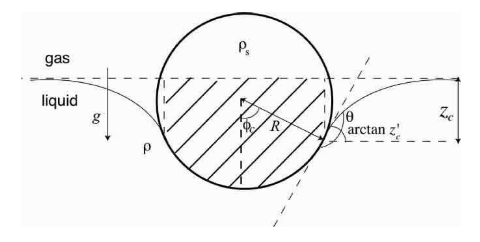
\includegraphics[width = 0.9\textwidth]{boulleflotantedecheerios.png}
        %     \caption{Geometry of a sphere lying at a liquid-gas interface. The shaded area represents the weight of liquid equivalent to the buoyancy force due to hydrostatic pressure acting on the sphere.\cite{vella_cheerios_2005}}
        % \end{figure}
        \begin{figure}[!htb]
            \centering
            \includegraphics[]{schema_geom_sphere_eau.tikz}
            \caption{Géométrie d'une sphère reposant sur une interface liquide-gaz. La partie rayée représente le poids de liquide équivalent à la force de flottabilité du à la pression hydrostatique appuyant sur la sphère. }
            \label{geom_sphere}
        \end{figure}

        Une des raisons pour laquelle les objets flottent est due à la poussée d'Archimède, comme nous pouvons le voir dans la figure \ref{geom_sphere}. Pour que notre sphère reste sur l'interface liquide-gaz elle a besoin que la norme de son poids \(||\vb*{P}||=\frac{4}{3}\pi\rho_{s}gR^3\); doit être équilibrée par la composante de tension superficielle agissant le long de la ligne de contact (circulaire) et par la force de flottabilité due au déplacement du fluide en vrac. La première composante a pour équation :

        \begin{equation}
            2\pi\gamma R\sin{\phi_c}\frac{z_c'}{\sqrt{1+z_c^{'2}}}
            \label{eq:tensionSuperficielle}
        \end{equation}

        Et nous avons également la force de flottabilité par l'équation :
        \begin{equation}
            \pi\rho_l g R^3 \left(\frac{z_c}{R}\sin^2{\phi_c} + \frac{2}{3}-\cos{\phi_c}+\frac{1}{3}\cos^3{\phi_c}\right)
            \label{eq:buoyancyForce}
        \end{equation}

        % TODO expiquer dou ca viens moi ja pas comprie
        % \begin{equation}
        %     2\pi R \phi_c \gamma \sin(\arctan z_c^{'}) = 2\pi\gamma R \sin\phi_c z_c^{'}(1+z_c^{'2})^{-1/2}
        %     \label{eq:wut}
        % \end{equation}

        Nous avons donc l'équilibre des forces donné par :
        \begin{equation}
            \frac{4}{3}\pi\rho_{s}gR^3 =2\pi\gamma R \sin\phi_c \frac{z_c^{'}}{\sqrt{(1+z_c^{'2})}} + \pi\rho_l g R^3 \left(\frac{z_c}{R}\sin^2 \phi_c + \frac{2}{3}-\cos\phi_c+\frac{1}{3}\cos^3 \phi_c\right)
            \label{eq:BalanceOfForces}
        \end{equation}

        % TODO cest quoi $z_c^{'}$??? Un point de contact apparemment 

        Si nous substituons \(\phi_c = \pi - \theta + \arctan z_c^{'}\) et gardons uniquement les termes linéaires en \(z_c^{'}\), nous retrouvons l'expression pour \(z_c^{'}\sin \phi_c\) qui est précis par rapport \textit{à l'ordre linéaire du nombre de Bond}, \(B \equiv R^2/L_c^2\) 

        Nous avons donc:
        \begin{equation}
            z_c^{'}\sin \phi_c = B\left(\frac{2D-1}{3}-\frac{1}{2}\cos \theta + \frac{1}{6} \cos^3 \theta\right) \equiv B\Sigma
            \label{eq:bondsigma}
        \end{equation}
        Avec \(D \equiv \frac{\rho_s}{\rho}\).

        % On peux voir ceci est bien le cas car on observe bien que \(z_c^{'} = 0\) quand \(\theta = \pi/2\) et \(D = 1/2\) cest ce que on satendais car dans ce cas la pousee de archimede seul lui meme est assez pour equilibrer le poids de la sphere sans deformations du liquide.

        L'équation (\ref{eq:bondsigma}) contient deux paramètres sans dimensions; \textit{le nombre de Bond} $B$ et $\Sigma$, qui sont très importants pour notre modélisation.

        Le nombre de Bond vaut:
        \begin{equation}
            B = \frac{(\rho_l-\rho_{a})gR^2}{\gamma} \simeq \frac{R^2}{L_c^2}
        \end{equation}

        Il nous donne la mesure relative de l'importance des effets de gravité et de la tension de surface; si $B$ est tres grand, cela correspond à des particules grandes ou à une tension de surface petite. 

        Pour déterminer $\Sigma$, nous avons besoin de l'angle de contact $\theta$. Pour le trouver nous avons suivi l'article \textit{Lattice Boltzmann Simulation of Capillary Interactions among Colloidal Particles}\cite{lattice_boltzmann_caplilary_interaction} dans lequel ils utilisent un angle de contact ($\theta$) satisfiant la loi de Young-Dupré supposant que les particules sont assez petites pour que nous puissions négliger les effets de leurs poids sur l'angle de contact. %TODO PAS DU TOUT SUR SI DANS LE NOTRE NOUS AVONS LE DROIT DE FAIRE COMME CA???? (EST QUE ON A UN AUTRE CHOIX ? NOPE :/ DONC ON FAIT TEL QUE CEST NEGLIGABLE DU COUP CEST POUR CA QUE IL NA PAS MARCHE AVEC LES PUNAISES???)
        \begin{equation}
            \cos \theta = \frac{\gamma_{SV}-\gamma_{SL}}{\gamma_{LV}}
            \label{eq:cos_angle_contact}
        \end{equation}
        Ou $\gamma_{SV,SL,LV}$ est la tension superficielle des interfaces Solide/Vapeur, Solide/Liquide et Liquide/Vapeur.
        Avec $\arctan z_c^{'} = \sin^{-1}\left(\frac{\pi}{2}B\right)$ \cite{lattice_boltzmann_caplilary_interaction}. 
        
        De ici on a besoin des tension superficielle expérimentale de chaque milieu ($\gamma_{SV, SL, LV}$) equation \ref{eq:cos_angle_contact} mais comme on a pas les valeurs expérimentale pour chaque objet par rapport aux milieux 
        \begin{equation}
            \theta \simeq \pi - \arctan z_c^{'}
        \end{equation}
        Qui nous donne un approximation
        % \begin{equation}
        %     \phi_c = \sin^{-1}\left(\frac{\pi}{2}B\right) = \pi - \theta + \arctan z_c^{'}
        %     \label{eq:phi}
        % \end{equation}
        % Si on combine les equations \ref{eq:bondsigma} et \ref{eq:phi} on a:
        % \begin{equation}
        %     z_c^{'} \sin \left(\sin^-1\left(\frac{\pi}{2}B\right)\right) = B \Sigma
        % \end{equation}
        % \begin{equation}
        %     \Rightarrow z_c^{'}\left(\frac{\pi}{2}B\right) = B \Sigma
        % \end{equation}
        % \begin{equation}
        %     \Rightarrow z_c^{'}\frac{\pi}{2} = \Sigma = \left(\frac{2D-1}{3}-\frac{1}{2}\cos \theta + \frac{1}{6} \cos^3 \theta\right)
        %     \label{eq:zcpi/2=sigma}
        % \end{equation}
        %  Si nous substions \(\phi_c =  \sin^{-1}\left(\frac{\pi}{2}B\right) = \pi - \theta + \arctan z_c^{'} \) On a:
        % \begin{equation}
        %     % \Rightarrow \theta = \pi - \sin^{-1}\left(\frac{\pi}{2}B\right) + \arctan z_c^{'}
        %     z_c^{'} = \tan\left(\sin^{-1}\left(\frac{\pi}{2}B\right)-\pi+\theta\right)
        %     \label{eq:thetafinaly?}
        % \end{equation}
        % Si on remplace le \(z_c^{'}\) dans l'equation \ref{eq:zcpi/2=sigma} avec lequation \ref{eq:thetafinaly} on a:
        % \begin{equation}
        %     \tan\left(\sin^{-1}\left(\frac{\pi}{2}B\right)-\pi+\theta\right)\frac{\pi}{2} =\frac{2D-1}{3}-\frac{1}{2}\cos \theta + \frac{1}{6} \cos^3 \theta 
        % \end{equation}
        % Si on applique deux fois l'egalite trigonometrique: 
        % \begin{equation}
        %     \tan (a+b) = \frac{\tan a + \tan b}{1-(\tan a \tan b)}
        % \end{equation}
        % A TESTER VOIR SI JE ME SUIS PAS TROMPE
        % \begin{equation}
        %     \Rightarrow \frac{\tan \phi_c + \tan (-\pi) + \tan\theta - (\tan \phi_c\tan (-\pi)\tan\theta)}{1-\tan \phi_c \tan(-\pi) - \tan\theta \tan\phi_c - \tan(-\pi)\tan\theta} = \Sigma 
        % \end{equation}
        % \(\tan(-\pi) = 0\)
        % \begin{equation}
        %     \Rightarrow \frac{\tan\phi_c + \tan\theta}{1-\tan\theta\tan\phi_c} = \frac{2D-1}{3}-\frac{1}{2}\cos \theta + \frac{1}{6} \cos^3 \theta
        % \end{equation}
        % Pour le reoudre a la main cest difficile mais numeriquement on peux avoir des solutions. On peux savoir la valeur de $\phi_c$ grace a l'equation \ref{eq:phi} et nous savons que \(D \equiv \frac{\rho_s}{\rho_l}\) alors on peux trouver $\theta$.
        % WUT ???
        % The expression for the slope of the interface in the vicinity of the spherical particle given in (9) is valid for B << 1 (corresponding to a radius of  1mm or smaller for a sphere at an air-water interface) in which case surface tension is very important. The other dimensionless parameter, , can be thought of as a (non-dimensional) resultant weight of the particle once the Archimedes upthrust has been subtracted out. This physical interpretation arises naturally from the vertical force balance condition (8) and (9) since the resultant weight of the object (in the linearised approximation) is simply 

        % L'expression de la pente de l'interface au voisinage de la particule sphérique donnée dans (\ref{eq:bondsigma}) est valable pour B << 1 (correspondant à un rayon de 1mm ou moins pour une sphère à l'interface air-eau), auquel cas la tension superficielle est très importante. L'autre paramètre sans dimension, peut être considéré comme un poids résultant (non dimensionnel) de la particule une fois que la poussée d'Archimède a été soustraite. Cette interprétation physique découle naturellement de la condition d'équilibre de la force verticale (\ref{eq:BalanceOfForces}) et (\ref{eq:bondsigma}) puisque le poids résultant de l'objet (dans l'approximation linéarisée) est simplement 

        %%%%%%%%%%%%%%%%%%%%%%%%%%%%%%%%%%%%%
        % To calculate the interaction energy using the Nicolson approximation, we must also calculate the interfacial displacement caused by an isolated floating sphere, which is determined by the hydrostatic balance \(\gamma\nabla^2h = \rho gh -\) the co-ordinate invariant statement of equation (1). With the assumption of cylindrical symmetry, this becomes:
        TODO EST QUEE CEST POSSIBLE DE METTRE UNE FIGURE ICI DUN TUBE AVEC DE LEAU QUE ON VOIS CEST QUOI H ET X ?
        Nous savons le déplacement interfacial\cite{introfluidcambridge} qui est:
        \begin{equation}
            \gamma \frac{\dd^2h}{\dd x^2} = \rho_l g h
        \end{equation}
        Si nous prenons en compte que l'objet a une symétrie sphérique
        \begin{equation}
            \Rightarrow \frac{1}{r} \frac{\dd}{\dd r} \left( r\frac{\dd h}{\dd r}\right) = \frac{h}{L_c^2}
        \end{equation}
        EN FAITE LASSOCIATIONAU FONCTION BESSEL CA VA MAIS JE SAIS PAS COMMENT PARTIR DE EQUATIONAVEC GAMMA ET DEDUIR UNE SYMETHRIE SPHERIQUE????\\
        Nous pouvons déduire une solution de cette équation avec la fonction de Bessel modifié à l'ordre 0 \cite{introbessel} $(K_0\left(\frac{l}{L_c}\right))$.

        \begin{figure}[H]
            \centering
            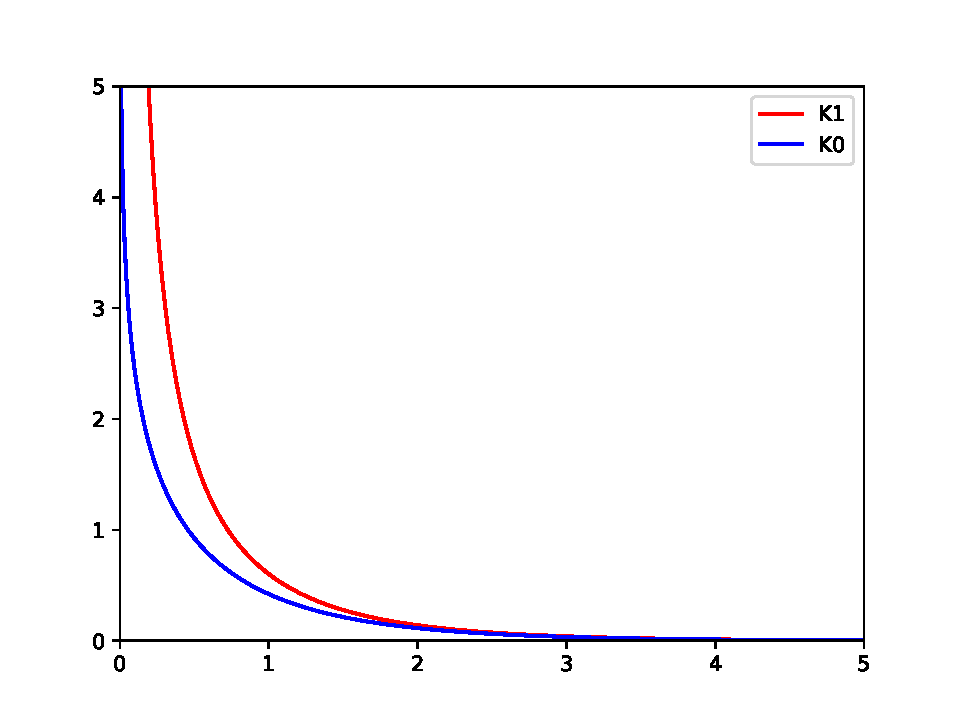
\includegraphics[width = 0.5\textwidth]{Besselk1_K0.pdf}
            \caption{Graphique représentant les fonctions de Bessel modifié à l'ordre 0 et 1}
            \label{fig:bessel}
        \end{figure}
        % TODO faire tel que on aligne a 0 le y et peut etre aller jusq a 6 en x ?
        %%%%%%%%%%%%%%%%%%%%%%%%%%%%%%%%%%%%

        Pour déterminer, maintenant la force d'attraction entre deux objets nous partons du poids effectif d'une sphère sur une interface déformé, que nous donnons comme \(2\pi RB\Sigma\). Nous avons également calculé la déformation interfaciale causée
        par la présence d'une seule sphère. Nous sommes donc capables de calculer l'énergie d'interaction entre deux sphères. Cette énergie est le produit du poids résultant d'une sphère et de son déplacement vertical causé par la présence d'une autre sphère dont le centre est éloigné de l'horizontale d'une distance horizontale $l$. Nous pouvons donc écrire l'énergie, $E(l)$, comme suit :
        \begin{equation}
            E(l)=-2\pi\gamma R^2b^2\Sigma^2K_0\left(\frac{l}{L_c}\right)
            \label{eq:energyInteraction}
        \end{equation}
        Avec $L_c$ la longueur capillaire.

        Nous pouvons donc trouver la force d'interaction $F(l)=-\frac{dE}{dl}$, ce qui donne :
        \begin{equation}
            \boxed{
                F(l)=-2\pi\gamma RB^{5/2}\Sigma^2K_1\left(\frac{l}{l_c}\right)
            }
            \label{eq:ForceInteraction}
        \end{equation}

        Nous voyons bien grâce a la Figure \ref{fig:bessel} que dès que $l/L_c>5$, notre force sera très faible et inversement quand $l/L_c << 1 $ la force d'attraction sera très élevée. La force entre objets flottants dépend donc de la distance entre eux, et cela de façon exponentiel.

        Nous avons décidé de ne pas prendre en compte les forces de frottement entre les objets et le liquide car elles étaient négligeables et elles auraient grandement complexifiées les calculs de notre algorithme.

        % TODO dans le code ajouter un buoyancy force qui calcule la ousee de archimede et dis si notre objet flotte ou pas si il flotte pas on peux metre un option tel quel il prend la valeur automatique ??? Ou on le neglige ????
        % TODO On mets les formules et peut etre demontrer ou ils viennent et surtout les cas ou on peux utiliser ces formules les cas ou ca marche pas etc\ldots
        % TODO SCHEMA deux cheeios et sur le schema on monre l Rayon de courbure etc...

        % TODO peut etre rephrase, lidee est la mais lexecution nest pas   
        %\newpage
        \subsection{Force des bords}
            \begin{wrapfigure}{r}{0.25\textwidth}
            \centering
                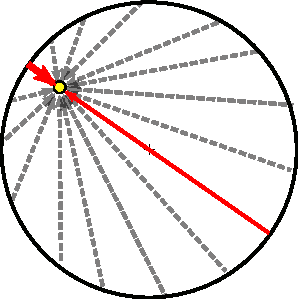
\includegraphics[width = 0.2\textwidth]{Figure_Force_Bord.pdf}
                \caption{Schéma des forces des bords.}
                \label{fig:Force_Bord_schéma}
            \end{wrapfigure}
            Maintenant que nous avons vu l'application des forces entre objets, nous allons expliquer les forces entre les bords et les objets. La force se calcule de la même manière qu'entre deux objets (equation \ref{eq:ForceInteraction}) car la force depend du rayon de courbure($R$), du nombre de Bond($B$), de Sigma($\Sigma$), de la longueur capillaire($L_c$) et de la distance entre deux points($l$) de force et tous ces paramètres peuvent être déterminer pour le bord. Pour la force appliquée par les bords sur les objets nous avons, à la place de calculer les forces à chaque point du cercle, opté d'utiliser la symétrie dun cercle. Nous avons remarqué que la plupart des forces s'annulent entre elles (en gris) et il nous reste seulement deux forces (en rouge) qui interagissent comme le montre la figure\ref{fig:Force_Bord_schéma}. Les seuls paramètres à changer sont le nombre de Bond et l'angle de contact, que nous prenons à 45 degré, angle du ménisque formé par l'eau dans un récipient en verre. 
            % Pour la force appliquée par les bords sur les objets nous avons décidé de ne pas calculer les forces de chaque point du bord, au lieu de cela nous avons utilisé la symétrie d'un cercle (nos bords étant un cercle). Seulement deux forces de bords vont s'appliquer sur un objet, les autres s'annulant par symétrie, comme le montre la figure \ref{fig:Force_Bord_schéma}
            % \begin{figure}[H]%[!htb]
            %     \centering
            %     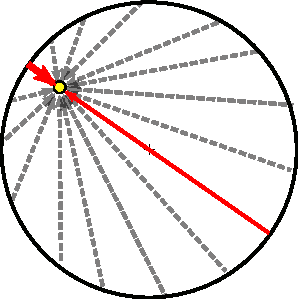
\includegraphics{Figure_Force_Bord.pdf}
            %     \caption{Schéma des forces des bords.}
            %     \label{fig:Force_Bord_schéma}
            % \end{figure}